% !TEX root = ../my-thesis.tex
%

\chapter{\textcolor{ctcolormain}{Introducción General}}\label{sec:intro}
\newpage

\section{Cambio climático y ecosistemas forestales}\label{sec:intro:climate-change}

En la actualidad existen evidencias científicas de los efectos del cambio global sobre los sistemas naturales \autocites{IPCC2013ClimateChange,HerreroZavala2015BosquesBiodiversidad}. Muchos procesos se están viendo alterados debido al cambio climático: cambios en el área de distribución de las especies \autocites{Thuilleretal2005ClimateChange}; alteraciones fenológicas \autocites{GordoSanz2005PhenologyClimate, EstiartePenuelas2015AlterationPhenology}, invasiones de especies \autocite{GonzalezMorenoetal14PlantInvasions}, aumento en la severidad e incidencia de plagas forestales \autocites{Hodaretal2012CambioClimatico,HodarZamora2004HerbivoryClimatic}, alteraciones en las interacciones ecológicas \autocites{MontoyaRaffaelli2010ClimateChange}, por citar algunos. Estos y otros cambios están modificando la composición, estructura y el funcionamiento de los ecosistemas, así como los bienes y servicios que éstos proporcionan \autocites{Dingetal2016ValuingClimate}. Para la región mediterránea, los efectos del cambio climático se espera que sean más severos que en otras regiones de la Tierra \autocites{Giorgi2006ClimateChange,IPCC2013ClimateChange} y en los ecosistemas forestales mediterráneos estos cambios tendrán impactos significativos \autocites{Regato2008AdaptingGlobal,RescodeDiosetal2006ClimateChange,Penuelasetal2017ImpactsGlobal,HerreroZavala2015BosquesBiodiversidad}.  

En la región Mediterránea se ha registrado en las últimas décadas un aumento generalizado de las temperaturas, así como un cambio en los patrones de precipitación \autocites{PerezBoscolo2010ClimateSpain,GiorgiLionello2008ClimateChange,Crameretal2020ClimateEnvironmental}. Para Sierra Nevada, usando datos datos de estaciones meteorológicas y mapas climáticos de alta resolución \autocites{Benitoetal2012SimulacionesClimaticas}, se han encontrado tendencias positivas para la temperaturas mínimas y máximas anuales, así como un patrón generalizado de reducción de la precipitación anual desde la década de 1960 \autocites{PerezLuqueetal2016SenalesCambio,PerezLuqueetal2021ClimaNevadaBase}.  

Una de las característica del cambio climático, además del aumento en las temperaturas y el cambio en el régime de precipitación, es el aumento de los eventos extremos, tales como sequías, tormentas, inundaciones, etc. \autocite{IPCC2013ClimateChange}. A pesar de que la sequía es una característica del clima mediterráneo \autocites{Lionello2012}, en las últimas décadas se ha registrado un incremento en la duración, frecuencia y severidad de los eventos de sequía \autocites{LloydHughesSaunders2002DroughtClimatology, Sousaetal2011TrendsExtremes,Colletal2017DroughtVariability}, particularmente en el sur de Europa \autocites{VicenteSerranoetal2014EvidenceIncreasing,Staggeetal2017ObservedDrought,Spinonietal2015EuropeanDrought,Pascoaetal2017DroughtTrends}, donde además se ha observado una tendencia hacia veranos más secos \autocites{Spinonietal2017PanEuropeanSeasonal}.  Este hecho cobra especial relevancia para el área Mediterránea, considerada una de las más vulnerables frente al cambio climático \autocites{Giorgi2006ClimateChange}, y donde las proyecciones a futuro pronostican un aumento de la severidad de los eventos climáticos extremos extremos \autocites{Hoerlingetal2012IncreasedFrequency,IPCC2013ClimateChange,Trenberthetal2014GlobalWarming,Spinonietal2018WillDrought}. En Sierra Nevada también se ha observado este patrón de incremento de sequías en las últimas décadas (\figreft{fig:intro:sequia})

\begin{figure}
	\centering
	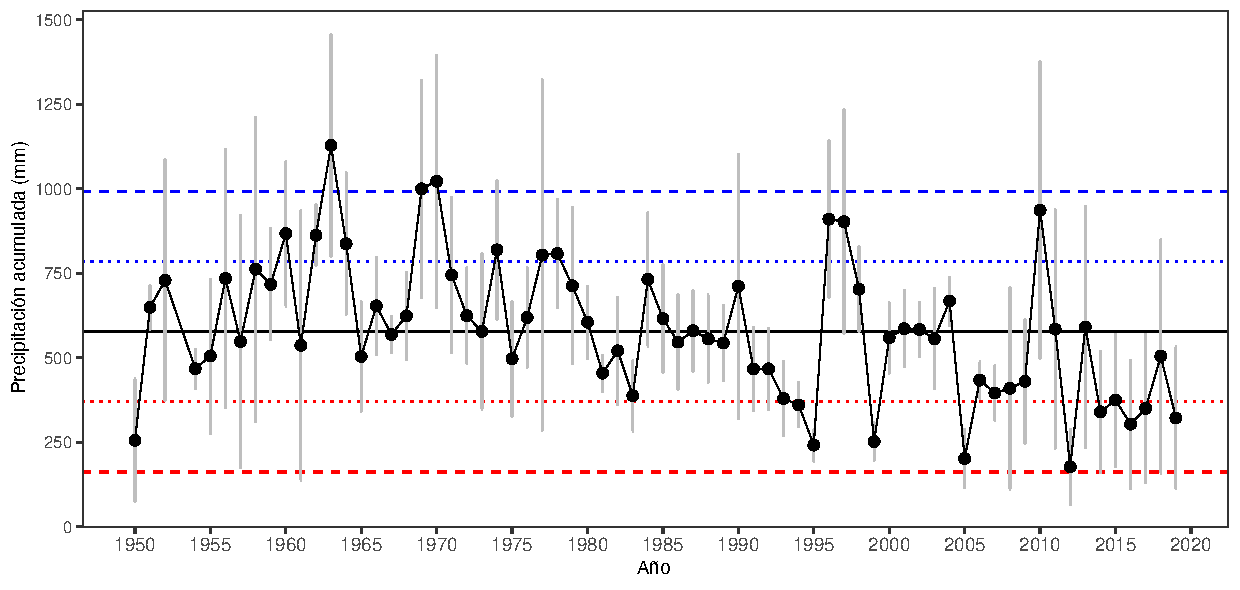
\includegraphics[width=\textwidth]{img/intro/intro-sequia.pdf} \caption{Evolución temporal de la precipitación acumulada (año hidrológico) durante el periodo 1950-2020 para Sierra Nevada (datos procedentes de 28 estaciones meteorológicas). Los puntos representan la media y las barras de error, el error estándar. La línea negra indica la precipitación acumulada media para todo el periodo (585 mm). Las líneas rojas representan -1 y -2 desviaciones estándar (líneas punteadas y discontinuas respectivamente). Las líneas azules representan +1 y +2 desviaciones estándar (líneas punteadas y discontinuas, respectivamente). Datos de \autocite{PerezLuqueetal2021ClimaNevadaBase}}\label{fig:intro:sequia}
\end{figure}

El incremento en la frecuencia y severidad de las sequías está alterando el funcionamiento de los ecosistemas mediterráneos a diferentes escalas \autocites{Penuelasetal2017ImpactsGlobal,Forneretal2018ExtremeDroughts,Liuetal2020EffectsDecadal,OgayaPenuelas2021ClimateChange}, puesto que la sequía afecta a aspectos fisiológicos, funcionales, estructurales y demográficos de los ecosistemas forestales \autocites{Allenetal2010GlobalOverview, Assaletal2016SpatialTemporal}. No obstante, se están observando respuestas divergentes de los ecosistemas forestales a la sequía \autocites{Andereggetal2020DivergentForest}, poniendo de manifiesto la importancia de otros aspectos como el momento en el que ocurre la sequía \autocites{Huangetal2018DroughtTiming}. Esto es de especial relevancia para especies de frondosas como el \Qpy que presenta una fenología de crecimiento bien marcada \autocites{PerezdeLisetal2016ChangesSpring}. 


Ahora estudios para esta especie ... 
Estudios de cambio climático en esta especie (ver ch1_potential_effects_climate_change.Rmd)



\section{Vivir en los márgenes}\label{sec:intro:rear-edge}

La hipótesis Centro-Periferia (\texbf{CPH} de su siglas en inglés, \textit{Centre-Periphery Hypothesi}) es un postulado biogeográfico que pretende explicar la variación de las características demográficas, genéticas y ecológicas de especies en sus áreas de distribución \autocite{Sextonetal2009EvolutionEcology, Pirononetal2015GeographicClimatic}. Esta hipótesis asume que el rango de una especie es una representación geográfica de su rango ecológico, y por tanto las condiciones ambientales son óptimas en el centro de su área de distribución y más severas en las regiones periféricas \autocite{Pirononetal2017GeographicVariation}(Figura). Así, las poblaciones situadas en la periferia geográfica experimentan condiciones ecológicas (abióticas y/o bióticas) más desfavorables que conducen a menor densidad de población y eficacia ecológica \autocite[\textit{fitness},][]{Brown1984RelationshipAbundance}. A medida que se alcanzan los límites de los recursos ecológicos de las especies, las poblaciones se vuelven más pequeñas y más aisladas espacialmente, y tienden a perder variación genética \autocites[][]{Karketal2008HowDoes,Garciaetal2010LivingEdge}. La hipótesis Centro-Periferia se ha utilizado ampliamente como base de diferentes hipótesis sobre procesos ecológicos y evolutivos, abordando desde el flujo genético entre poblaciones a otras cuestiones más aplicadas como la forma en la que las poblaciones responderán al cambio climático \autocites{SagarinGaines2002AbundantCentre}. 

Tradicionalmente se ha considerado que las poblaciones situadas en los márgenes de su rango de distribución presentan un peor rendimiento y son más vulnerables que las situadas en el centro de su distribución, sin embargo en los ultimos años se ha observado cómo algunos rasgos funcionales (\emph{e.g.} supervivencia, fecundidad) no siempre siguen las predicciones de esta hipótesis \autocite{Pirononetal2017GeographicVariation}. De hecho, en varios trabajos de revisión donde se realiza una compilación de estudios de ecología y evlución basados en el supuesto de la hipótesis centro-periferia de \autocites{SagarinGaines2002AbundantCentre,Pirononetal2017GeographicVariation}, se encontraron evidencias empíricas a favor de la hipótesis centro-periferia para entre un 40\% y un 50\% de los estudios analizados. 

Mete la revisión genética de Ecket 
...

Ahora poner un par de ejemplos de cuando no se cumple para especies forestales ... 


Así por ejemplo, se han observado tendencias de crecimiento mas positivas en poblaciones de \emph{Pinus sylvestris} situadas en el rear-edge de su distribución que en las zonas centrales y en las zonas de latitudes más al norte \autocite{Matiasetal2017ContrastingGrowth}. 


Todo ello ha llevado a que varios autores apunten la necesidad de redefinir esto (VIla Cabrera ....) 


Las poblaciones localizadas en el frente de retroceso \autocite[\textit{rear-edge, sensu} ][]{HampePetit2005ConservingBiodiversity} son desproporcionadamente importantes para la conservación a largo plazo de la diversidad genética de la especie, así como para la historia filogeográfica y el potencial evolutivo de la especie \autocite[][]{HampePetit2005ConservingBiodiversity}.  

Además 
GLOBAL CHANGE AND RANGE LIMITS
Additionally, rapid climate shifts will provide “opportunities” to examine the dynamics of expanding versus trailing range limits and the role of peripheral populations in conservation biology.




Muchas de las poblaciones situadas en sus bordes de distribución equatorial, han persistido a varias glaciaciones, suelen ser poblaciones relictas, y generalmente se situan en zonas con alta heterogeneidad de factores edáficos y topográficos, lo que les ha permitido responder a los cambios ambientales con migraciones pequeñas 


Esto es especialmente importante para las poblaciones que se sitúan en su borde-trasero de distribución en zonas aisladas de montaña. 

### Las montañas como estudio del cambio global. 



\section{Cambios de uso y montañas}
Los robledales, al igual que otras formaciones forestales, han sido objeto de intensas presiones de origen antrópico que han provocado la reducción de su área de distribución, así como la modificación en sus patrones florísticos y estructurales \autocites{Gavilanetal2000EffectsDisturbance,Gavilanetal2007ModellingCurrent,Tarregaetal2006ForestStructure}. 

Históricamente se han explotado en monte bajo para la obtención de leñas, carbón, taninos y producción de casca \autocite{RuizdelaTorre2006FloraMayor}. También se han llevado a cabo clareos para crear pastos con bajas densidades de árboles maduros que proporcionan bellotas, leñas y amplias áreas para el pastoreo e incluso a veces se quemaban para crear áreas de pastoreo \autocite{ValbuenaCarabanaGil2017CentenaryCoppicing}. De hecho, el sobrepastoreo en estas formaciones provocaba unas importantes pérdidas de suelo, aspecto que se viene señalando por los gestores forestales desde final del siglo XIX \autocite{Laguna1872ComisionFlora}. Todos estos procesos antropogénicos han transformado tanto las estructuras de los robledales, que es difícil encontrar rodales que puedan considerarse como bosques naturales \autocite{RuizdelaTorre2006FloraMayor}. 

Esta presión antrópica también se ha observado en los robledales de Sierra Nevada \autocite{JimenezOlivencia1991PaisajesSierra}, donde el intenso aprovechamiento ganadero y forestal, la roturación de espacios para nuevos cultivos y pastos, la explotación de leña para uso doméstico o industrial, e incluso los incendios forestales, han ocasionado la reducción de la superficie que ocupaban estas formaciones \autocite{CamachoOlmedoetal2002AltaAlpujarra} (\figreft{fig:intro:usos}. Así por ejemplo, el melojar de la Solana de la Dehesa de San Jerónimo, sufrió una tala masiva en la posguerra para utilizar la leña como gasógeno para los automóviles \autocite{Prieto1975BosquesSierra}. En algunas zonas, la presión antrópica ha sido tan intensa, que se perdió por completo la cubierta forestal, lo que ocasionó graves problemas de erosión \autocite{MesaGarrido2019ReforestacionSilvicultura,RomeroZurbano1909DivisionHidrologicoforestal}. 

Todas estas actuaciones condujeron a una sobreexplotación de los robledales cuya configuración actual en Sierra Nevada parece depender, al igual que otras formaaciones vegetales, del uso del pasado \autocite{NavarroGonzalezetal2013WeightLanduse}. Sin embargo, a partir de la segunda mitad del siglo XX se produjo un abandono rural que produjo una disminución de la presión antrópica sobre los ecosistemas forestales. 

\begin{figure}
	\centering
	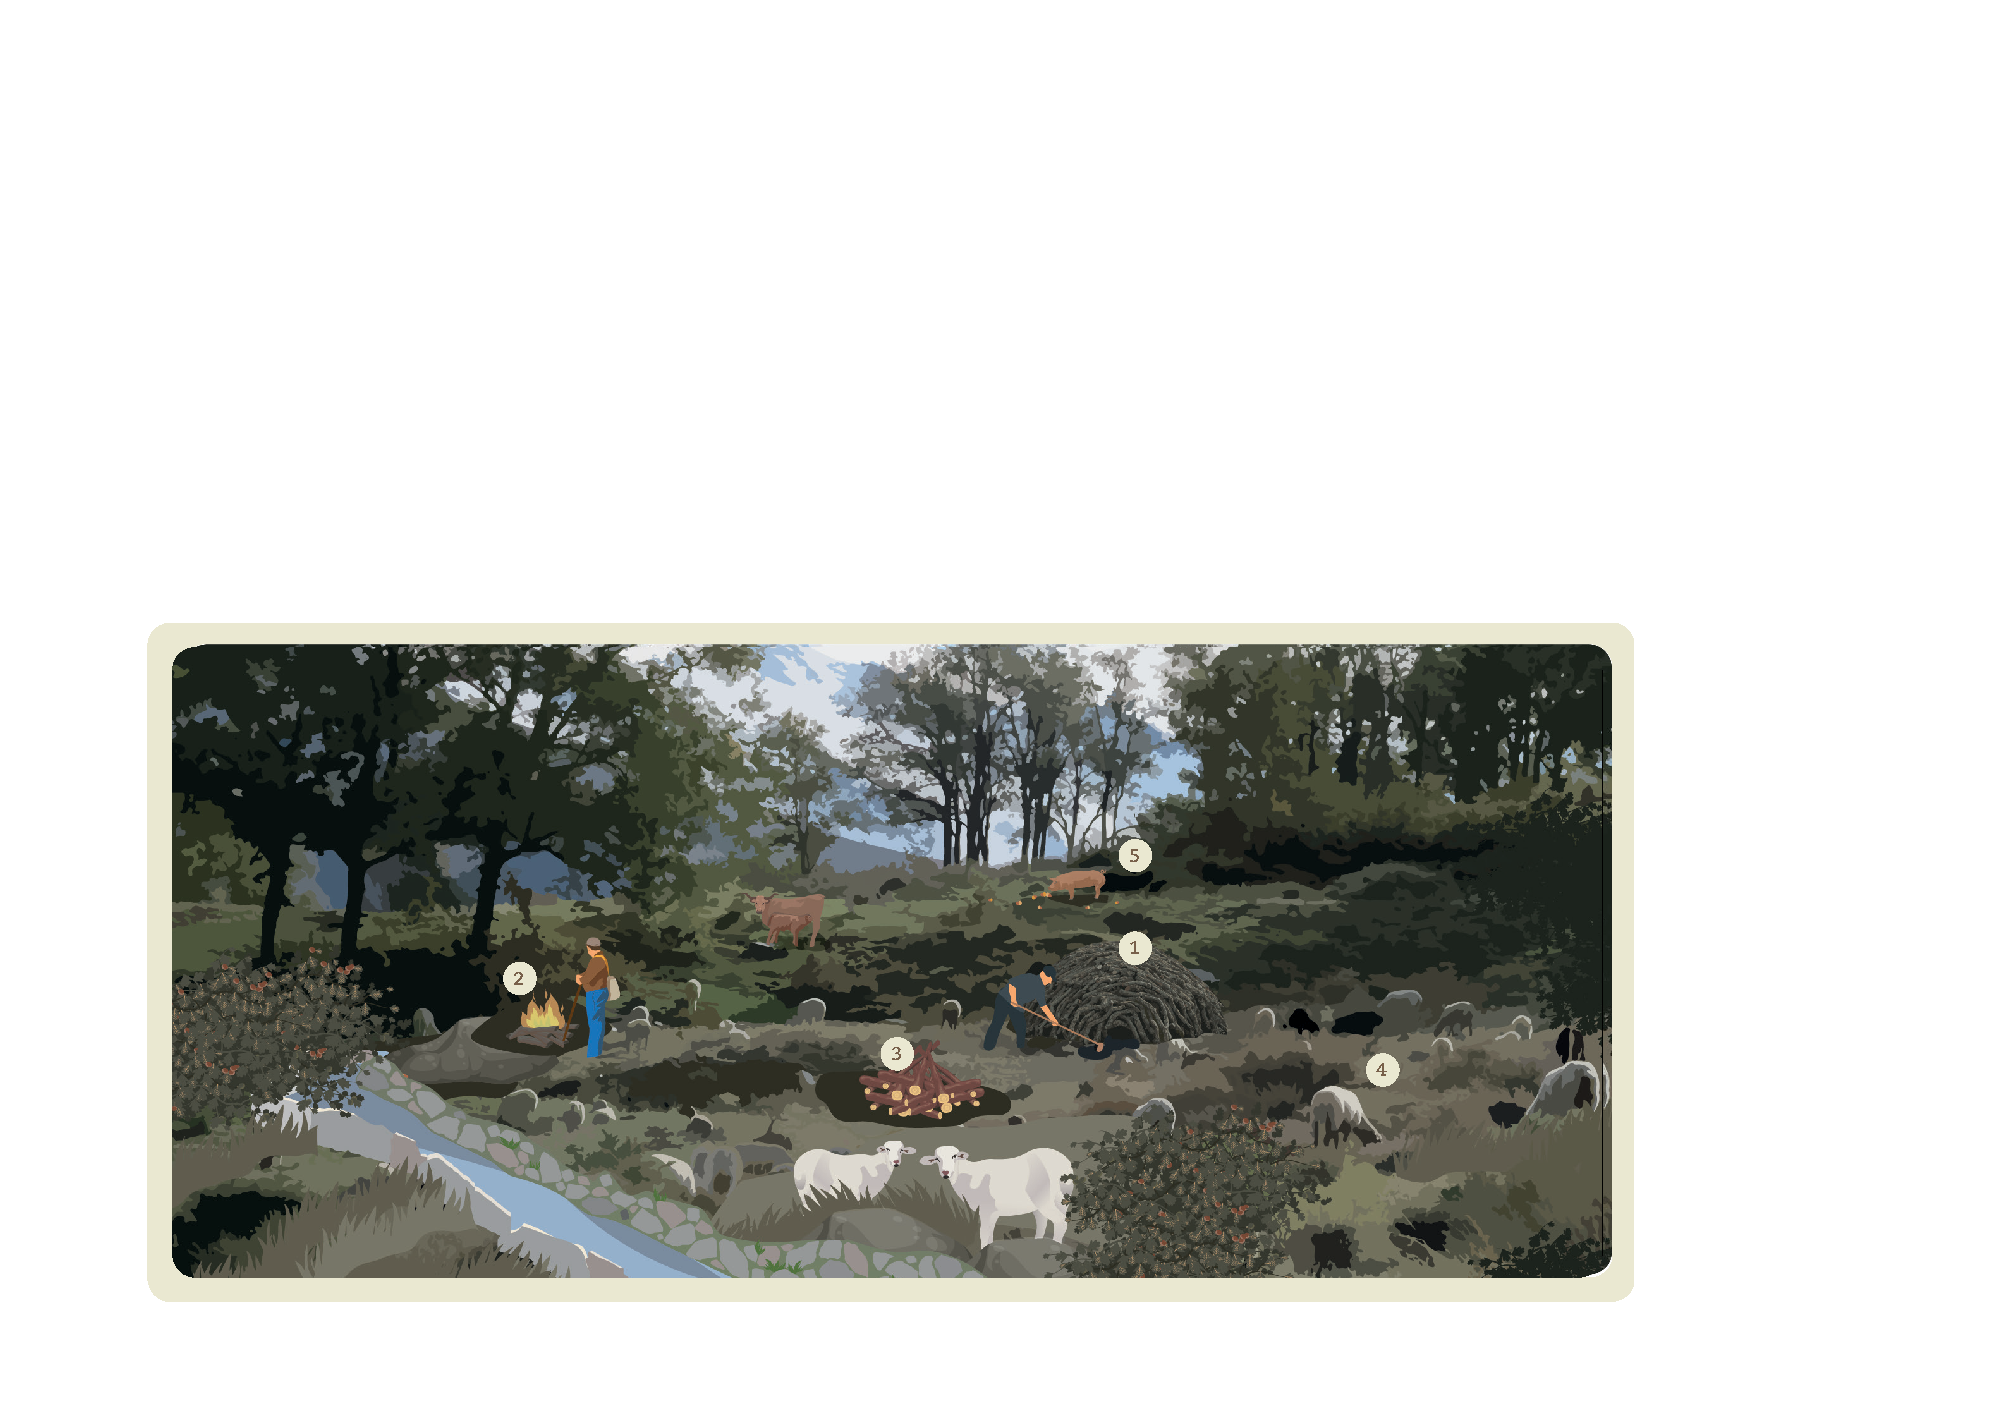
\includegraphics[width=\textwidth]{img/intro/intro-usos.pdf} \caption{Principales usos antrópicos del robledal. Pilas de leña para carboneo tradicional (1); quemas para la creación de áreas de pastoreo y cultivos (2); leñas para uso doméstico (3); pastoreo (4); y producción de bellotas (5).}\label{fig:intro:usos}
\end{figure}

\section{Objetivos}

Los objetivos de la presente memoria doctoral son: 

\paragraph{\emph{Caracterización ambiental de los robledales de Sierra Nevada}} \mbox{} \\
Realizaremos una caracterización ambiental del sistema de estudio (robledales) en Sierra Nevada. Queremos conocer el comportamiento de las diferentes poblaciones de robledal respecto a variables ambientales (climáticas, topográficas, etc.), composición, atributos forestales (estructurales) y funcionales. Concretamente, se pretende:

\begin{itemize}
	\item Caracterizar los robledales nevadenses respecto a variables abióticas y de estructura del bosque.
	\item Establecer los valores que definen el hábitat óptimo y marginal de las poblaciones de roble en Sierra Nevada.
	\item Identificar las variables abióticas que explican la distribución de los robledales en Sierra Nevada.
	\item Una vez identificadas las variables abióticas que condicionan la distribución de los robledales, nos interesa conocer si existen diferentes grupos determinados por variables abióticas. Intentaremos responder a la pregunta ¿que variables abióticas, o combinación de las mismas, discriminan mejor entre las poblaciones de robledal en Sierra Nevada?.
	\item Analizar si la discriminación en diferentes grupos, basada en características ambientales, se refleja en una discriminación basada en la composición de especies de las diferentes poblaciones así como de la estructura (atributos forestales) y el funcionamiento (regeneración y productividad). Es decir, ¿hay relación entre el agrupamiento basado en factores abióticos y el agrupamiento de composición, estructural y funcional?. 
\end{itemize}

\paragraph{\emph{Análisis del proceso de colonización de hábitats degradados próximos a las masas de robledal en Sierra Nevada}}\mbox{} \\
Queremos analizar el proceso de colonización de hábitats degradados (campos de cultivo abandonados) próximos a los robledales y explorar si existen diferencias entre las poblaciones en el límite sur de su distribución. Para ello nos enfocaremos en diferentes aspectos del proceso de colonización. En primer lugar analizaremos la estructura de la fuente semillera (bosque) para explorar diferencias entre las poblaciones situadas en la zona norte y las situadas en la zona sur. También evaluaremos la evolución de las poblaciones del principal vector dispersante del roble, el arrendajo (\emph{Garrulus glandarius}). Finalmente analizaremos el proceso de colonización en sí, es decir, los patrones de regeneración de robledal en diferentes cultivos abandonados, localizados en zonas cercanas a las poblaciones de robledal.
Al final conoceremos mas en profundidad como es el patrón de colonización de hábitats marginales por parte del robledal y si existen diferencias entre las diferentes poblaciones. Comprender la expansión de los robledales hacia áreas márginales (cultivos abandonados) es crítico para poder desarrollar estrategias de gestión efectivas de los robledales.


\paragraph{Cuantificación del papel de los robledales de Sierra Nevada como sumidero de carbono y análisis de la tendencia temporal} \mbox{} \\
El secuestro de carbono es uno de los servicios ecosistémicos más relevantes que proporcionan los bosques mediterráneos, siendo un indicador de la capacidad del ecosistema para contribuir a la regulación del clima. Los robledales, como ecosistemas mediterráneos representan un sumidero de carbono. El objetivo de este capítulo es cuantificar la capacidad  de secuestro de carbono de los robledales de Sierra Nevada, situados en el borde de su distribución, explorando las posibles diferencias entre las poblaciones de robledal dentro de esta región montañosa. Asimismo estamos interesados en analizar la evolución temporal de este servicio ecosistémico 

\paragraph{Efectos del cambio climático en la productividad de los robledales en Sierra Nevada}\mbox{} \\
Se trata de evaluar como alteraciones en los patrones de disponibilidad hídrica debido al cambio climático pueden afectar a la productividad de esta formación forestal. Conocemos que los robledales presenta una estación de crecimiento bien definida y centrada en verano . Por ello es de interés evaluar la productividad de los robledales (utilizando índices de vegetación obtenidos a partir de imágenes de satélite) frente a cambios en los patrones de disponibilidad hídrica. Nos centraremos en analizar modificaciones en la cantidad de agua (disminución de la disponibilidad de agua debido a eventos de sequía) así como alteraciones en la distribución temporal de la disponibilidad de agua (\emph{p.ej.}: adelantos en la fusión de la cubierta de nieve).

\paragraph{Resiliencia de los robledales frente a la sequía}\mbox{} \\
El cambio global supone un reto para los ecosistemas forestales localizados en el borde de su distribución debido a su vulnerabilidad a los eventos de sequía 

a que además del uso antrópico al que han estado sometidos 

a la sequía además los ecosistemas han estado sometido a un uso antrópico intensivo. 

Nuestro objetivo es analizar la resiliencia a la sequía de las poblaciones relictas de \Qpy localizados en el sur de la Península Ibérica 


\paragraph{Identificación de los servicios ecosistémicos proporcionados por los robledales}\mbox{} \\

Los ecosistemas forestales proporcionan diversos servicios ecosistémicos. 

... 
